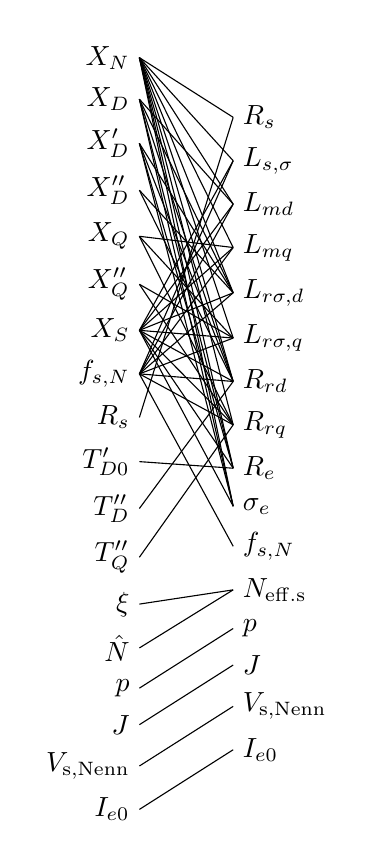
\begin{tikzpicture}[node distance=.5cm]
    % Linke Seite
    \begin{scope}[]
    	    \matrix[column 1/.style={anchor=base east}]{
             \node[] (XN) {$X_N$}; \\
             \node[] (XD) {$X_D$}; \\
             \node[] (XD') {$X_D'$}; \\
             \node[] (XD'') {$X_D''$}; \\
             \node[] (XQ) {$X_Q$}; \\
             \node[] (XQ'') {$X_Q''$}; \\
             \node[] (XS) {$X_S$}; \\
             \node[] (fsNl) {$f_{s,N}$}; \\
             \node[] (Rsl) {$R_s$}; \\
             \node[] (TD0') {$T_{D0}'$}; \\
             \node[] (TD'') {$T_D''$}; \\
             \node[] (TQ'') {$T_Q''$}; \\
             \node[] (xi) {$\xi$};\\
             \node[] (N) {$\hat N$};\\
             \node[] (pl) {$p$};\\
             \node[] (Jl) {$J$};\\             
             \node[] (VsNennl) {$V_{\mathrm{s,Nenn}}$};\\
             \node[] (Ie0l) {$I_{e0}$};\\
        };
    \end{scope}
    % Rechte Seite
    \begin{scope}[xshift=2.5cm]
    	    \matrix[column 1/.style={anchor=base west}]{
             \node[] (Rs) {$R_s$}; \\
             \node[] (Lssigma) {$L_{s,\sigma}$}; \\
             \node[] (Lmd) {$L_{md}$}; \\
             \node[] (Lmq) {$L_{mq}$}; \\
             \node[] (Lrsigmad) {$L_{r\sigma,d}$}; \\
             \node[] (Lrsigmaq) {$L_{r\sigma,q}$}; \\
             \node[] (Rrd) {$R_{rd}$}; \\
             \node[] (Rrq) {$R_{rq}$}; \\
             \node[] (Re) {$R_e$}; \\
             \node[] (sigmae) {$\sigma_e$};\\
             \node[] (fsN) {$f_{s,N}$}; \\
             \node[] (Neff) {$N_{\mathrm{eff.s}}$};\\
             \node[] (p) {$p$};\\
             \node[] (J) {$J$};\\
             \node[] (VsNenn) {$V_{\mathrm{s,Nenn}}$};\\
             \node[] (Ie0) {$I_{e0}$};\\
        };
    \end{scope}
    \draw (XN.east) edge (Rs.west)
               edge (Lssigma.west)
               edge (Lmd.west)
               edge (Lmq.west)
               edge (Lrsigmad.west)
               edge (Lrsigmaq.west)
               edge (Rrd.west)
               edge (Rrq.west)
               edge (Re.west)
               edge (sigmae.west);

    \draw (XD.east) edge (Lmd.west)
               edge (Lrsigmad.west)
               edge (Rrd.west)
               edge (Re.west)
               edge (sigmae.west);
               
    \draw (XD'.east) edge (Lrsigmad.west)
                edge (Rrd.west)
                edge (Re.west)
               edge (sigmae.west);
                
    \draw (XD''.east) edge (Lrsigmad.west)
                 edge (Rrd.west);
                 
    \draw (XQ.east) edge (Lmq.west)
               edge (Lrsigmaq.west)
               edge (Rrq.west);
               
    \draw (XQ''.east) edge (Lrsigmaq.west)
                 edge (Rrq.west);
                 
    \draw (XS.east) edge (Lssigma.west)
               edge (Lmd.west)
               edge (Lmq.west)
               edge (Lrsigmad.west)
               edge (Lrsigmaq.west)
               edge (Rrd.west)
               edge (Rrq.west)
               edge (Re.west)
               edge (sigmae.west);
               
    \draw (fsNl.east) edge (Lssigma.west)
                edge (Lmd.west)
                edge (Lmq.west)
                edge (Lrsigmad.west)
                edge (Lrsigmaq.west)
                edge (Rrd.west)
                edge (Rrq.west)
                edge (fsN.west);
                
    \draw (Rsl.east) edge (Rs.west);
    
    \draw (TD0'.east) edge (Re.west);
    
    \draw (TD''.east) edge (Rrd.west);
    
    \draw (TQ''.east) edge (Rrq.west);
    
    \draw (xi.east) edge (Neff.west);
    
    \draw (N.east) edge (Neff.west);

    \draw (pl.east) edge (p.west);
    
    \draw (Jl.east) edge (J.west);
    
    \draw (VsNennl.east) edge (VsNenn.west);
    
    \draw (Ie0l.east) edge (Ie0.west);    
\end{tikzpicture}

%             \node[] (XN) {$X_N$}; \\
%             \node[below=of XN] (XD) {$X_D$}; \\
%             \node[below=of XD] (XD') {$X_D'$}; \\
%             \node[below=of XD'] (XD'') {$X_D''$}; \\
%             \node[below=of XD''] (XQ) {$X_Q$}; \\
%             \node[below=of XQ] (XQ'') {$X_Q''$}; \\
%             \node[below=of XQ''] (XS) {$X_S$}; \\
%             \node[below=of XS] (fsN) {$f_{s,N}$}; \\
%             \node[below=of fsN] (Rs) {$R_s$}; \\
%             \node[below=of Rs] (TD0') {$T_{D0}'$}; \\
%             \node[below=of TD0'] (TD'') {$T_D''$}; \\
%             \node[below=of TD''] (TQ'') {$T_Q''$}; \\